\graphicspath{{Introduction/Figs/}}

\chapter{Introduction}

\section{Introduction to single-cell sequencing}

Next-generation sequencing technologies have revolutionised the study of biological systems by enabling the genome-wide profiling of molecular layers in un unbiased manner, including the genome \cite{Fleischmann1995} the epigenome \cite{Frommer1992} and the transcriptome \cite{Lister2008,Bainbridge2006,Nagalakshmi2008,Mortazavi2008}, among others. However, bulk sequencing approaches rely on a large number of cells to report an average molecular readout, and are hence limited for the study of complex biological processes where heterogeneity is expected at single cell resolution \cite{Griffiths2018,Papalexi2017,Patel2014}. The progressive development of low-input sequencing techniques resulted in an explosion of single-cell sequencing technologies, mostly for the transcriptome. In contrast to bulk protocols, single-cell techniques provide an unprecedented opportunity to study the molecular variation associated with cellular heterogeneity, lineage diversification and cell fate commitment \cite{Kolodziejczyk2015}.

The field of single-cell sequencing has largely been driven by the quantification of the messenger RNA (mRNA). In less than a decade, the field of single-cell transcriptomics has experienced an exponential growth of scale, driven by incremental optimisations of reagent volumes and consumable costs, as well as profound changes in the nature of the technology \cite{Svensson2018}. The earliest high-throughput single-cell RNA sequencing (scRNA-seq) technologies were published between 2009 and 2011, yielding a handful of cells. In 2019, there are studies that have achieved the astonishing milestone of profiling the transcriptome for more than a million cells in a single experiment \cite{Cao2019}. With the development of efficient commercial platforms, the maturation of scRNA-sequencing technologies has provided major insights on the study of lineage diversification and cell fate commitment \cite{Kolodziejczyk2015,Griffiths2018,Papalexi2017,Patel2014}. In 2020, we are at the stage of a major endeavour to generate transcriptomic atlases for different tissues, embryos and even entire adult organisms. The most ambitious of all is the Human Cell Atlas, aimed at building a reference map for all cells in the human body \cite{Aviv2017}.

\subsection{Single-cell RNA sequencing} \label{section:rna_expresssion}

scRNA-seq protocols differ extensively in terms of scalability, costs and sensitivity \cite{Svensson2018, Lafzi2018}. Broadly speaking, they can be classified into plate-based and droplet-based methods. In plate-based methods such as CEL-seq \cite{Hashimshony2012} and Smart-seq \cite{Ramskold2012, Picelli2014}, cells are isolated using micropipettes or flow cytometry into individual wells of a plate, where the library preparation is performed. Although plate-based strategies have limitations in terms of throughput and scalability, their main advantage is the higher quality of libraries and the full length transcript information (in the case of Smart-seq) which enables a more accurate quantification of splice variants \cite{Huang2017}, allele-specific expression \cite{Deng2014} and RNA velocity information \cite{LaManno2018}.
	
Droplet-based methods are based on the use of droplet microfluidics technology \cite{Zhang2019}. By capturing cells in individual droplets, each containing all necessary reagents for library preparation, this protocol allows the profiling of thousands of cells in a single experiment. These class of methods include InDrop \cite{Klein2015,Zilionis2016}, Drop-seq \cite{Macosko2015} and the comercial 10x Genomics Chromium \cite{Zheng2017}. As a trade-off, the increased high throughput of droplet-based approaches comes at the expense of reduced sensitivity \cite{Ziegenhain2017,Wang2019a,Svensson2017}.

More recently, a third type of scRNA-seq methodology emerged based on a combinatorial cellular indexing strategy \cite{Cao2017,Rosenberg2018,Cao2019}, which has permitted the sequencing of more than a million cells in a single experiment for a fraction of the cost of other methods, albeit a the cost of much lower sensitivity.

\subsection{Single-cell sequencing of the epigenome}

While the large majority of single-cell studies are focused on quantifying RNA expression, transcriptomic readouts provide a single dimension of cellular heterogeneity and hence contain limited information to characterise the molecular determinants of phenotypic variation \cite{Ritchie2015}. Consequently, gene expression markers have been identified for a myriad of biological systems, but the role of the accompanying epigenetic changes in driving cell fate decisions remains poorly understood \cite{Griffiths2018,Kelsey2017,Bheda2014}. Significant effort has been placed to obtain epigenetic measurements at single-cell resolution by adapting bulk methods to low-input material, a strategy thas has been successful for a variety of molecular layers, including chromatin accessibility \cite{Cusanovich2015,Cao2018,Chen2018}, DNA methylation \cite{Smallwood2014}, histone modifications \cite{Ku2019}, chromatin conformation \cite{Ku2019}, proteomics \cite{Specht2018} and lipidomics \cite{Thiele2019}, among others.

\subsubsection{DNA methylation} \label{section:dna_methylation}

DNA methylation is a stable epigenetic modification that is strongly associated with transcriptional regulation and lineage diversification in both developmental and adult tissues \cite{Jin2018, Harrison2011, Lee2014, Smith2013}. Its classical roles include the silencing of repetitive elements, inactivation of the X chromosome, gene imprinting, and repression of gene expression \cite{Jones2012}. Consistently, the disruption of the DNA methylation machinery is associated with multiple dysfunctions, including cancer \cite{Baylin2011}, autoimmune diseases \cite{Liu2013} and neurological disorders \cite{Amir1999}.
% In mammalian genomes, DNA methylation predominantly occurs at CpG dinucleotides (mCG). The presence of DNA methylation in non-CpG contexts (mCH) has been confirmed, albeit its functional role remains controversial \cite{He2015, Ramsahoye2000, Lister2009}.

% The establishment of DNA methylation signatures begin during development by the interplay of \textit{de novo} methylation and demethylation events. In mammals, methylation events are orchestrated by three different DNA methyltransferase enzymes with similar structure but different activity patterns: Dnmt1, Dnmt3a, Dnmt3b.
Protocols for the profiling of DNA methylation in single cells have emerged from its bulk counterparts, most notably bisulfite sequencing (BS-seq) \cite{Smallwood2014,Guo2013,Gravina2016,Farlik2015}. The underlying principle of BS-seq is the treatment of the DNA with sodium bisulfite before DNA sequencing, which converts unmethylated cytosine (C) residues to uracil (and eventually to thymine (T), after PCR amplification), leaving 5-methylcytosine residues intact. The resulting C$\to$T transitions can then be detected by DNA sequencing \cite{Frommer1992,Clark2016,Clark2017}. Nevertheless, the high degree of DNA degradation caused by the purification steps and the bisulfite treatment impaired the use of conventional BS-seq with low starting amounts of DNA. To address this problem, \cite{Smallwood2014} adapted the post-bisulfite adaptor tagging (PBAT) protocol with multiple rounds of 3' random primer amplification. When the bisulfite treatment is performed before ligation of adaptors, rather than afterwards, loss of adapter-tagged molecules is minimised, demonstrating the potential to use scBS-seq from low-input material. 
%In a proof of concept study, \cite{Smallwood2014} applied scBS-seq on ovulated metaphase II oocytes and mouse ESCs, reporting an average coverage of 3.7 million CpG dinucleotides (17.7\%) per cell.

% \begin{figure}[H]
% 	\centering
% 	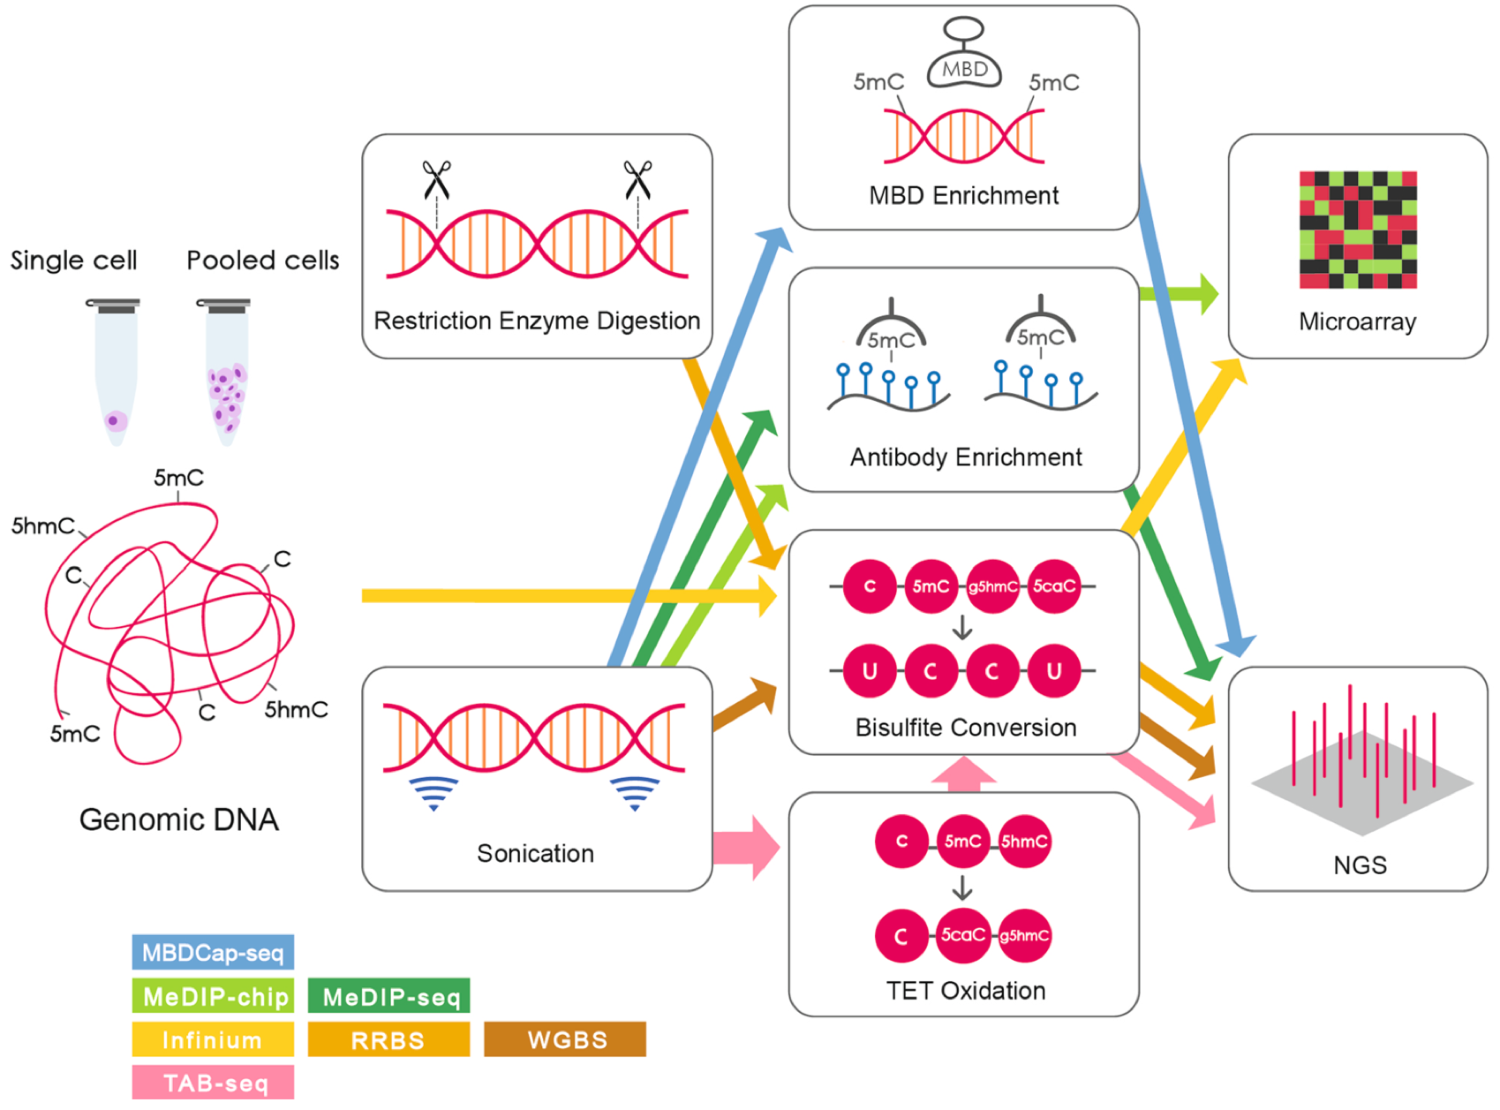
\includegraphics[width=0.8\linewidth]{methylation_protocols}
% 	\caption[]{Workflow of DNA methylation profiling protocols. Reprinted from \cite{Yong2016}}
% 	\label{fig:methylation_protocols}
% \end{figure}

% Alongside scBS, other bulk sequencing methods were also adapted to the single cell resolution, with different trade-offs between coverage and costs. For instance, \cite{Guo2015} adapted the reduced-representation bisulfite sequencing (RRBS-seq) to low starting material by performing all experimental steps before PCR amplification in a single tube. The key principle behind RRBS-seq is to digest the DNA with a restriction endonuclease, followed by a size-selection strategy to enrich for CpG-dense areas \cite{Meissner2005}. This approach significantly reduces sequencing costs at the expense of low coverage in CpG-poor genomic areas, which include repetitive elements, gene bodies and enhancer elements.

\subsubsection{Chromatin accessibility} \label{section:chromatin_accessibility}

In eukaryotes, the genome is packed into a compact complex of DNA, RNA and proteins called chromatin. Several layers of chromatin condensation have been identified, the fundamental unit being the nucleosome, which consists of a string of $\approx$  150bp of DNA wrapped around histone proteins, with linker DNA of $\approx$ 80bp connecting them \cite{Klemm2019,Tsompana2014}. The positioning of the nucleosomes in the nucleus provide an important layer of gene regulation, mostly by exposing or sheltering transcription factors binding sites \cite{Jiang2009}. In general, active regulatory regions tend to have low occupancy of nucleosomes, whereas inactive regions show a high density of nucleosomes \cite{Struhl2013}. Thus, the profiling of DNA accessibility and transcription factor footprints represents an important dimension to understand the regulation of gene expression.

% The N-terminal tails of the histones emerge from the nucleosome and are a strong hotspot for chemical modifications, including methylation, acetylation, phosphorylation and others \cite{Bannister2011}. The complex interaction between a histone modification and the corresponding position, often called the histone code, is an important driver of epigenetic regulation and an active area of research \cite{Zhao2015}.

Traditionally, three main experimental approaches have been used to map bulk chromatin accessibility in a genome-wide and high-throughput manner \cite{Nordstrom2019} (\Cref{fig:ChromatinAcc_protocols}): DNase sequencing (DNase-seq) \cite{Song2010}, transposase-accessible chromatin followed by sequencing (ATAC-seq) \cite{Buenrostro2013} and Nucleosome Occupancy and Methylome-sequencing (NOMe-seq) \cite{Kelly2012}.

\begin{itemize}

	\item \textbf{DNase-seq}: cells are incubated with DNAse I, an enzyme that in low concentrations cuts nucleosome-free regions, hence releasing accessible sites that are subsequently sequenced \cite{Song2010}. Although this methodology became one of the gold standards to map chromatin accessibility by the ENCODE consortium \cite{ENCODE2012,Thurman2012}, it has now been reported that DNase I introduces significant cleavage biases, thus affecting its reliability to infer transcription factor footprints \cite{He2013}.

	\item \textbf{ATAC-seq}: cells are incubated with hyperactive mutant Tn5 transposase, an enzyme that inserts artifical sequencing adapters into nucleosome-free regions. Subsequently, the adaptors are purified, PCR-amplified  and sequenced. In the recent years it has displaced DNase-seq as the \textit{de facto} method for profiling chromatin accessibility due to its fast and sensitive protocol \cite{Buenrostro2015b,Tsompana2014}.

	\item \textbf{NOMe-seq}: follows a very different strategy than the previous technologies. Cells are incubated with a GpC methyltransferase (M.CviPI), which labels accessible (or nucleosome depleted) GpC sites by DNA methylation. In mammalian genomes, cytosine residues in GpC dinucleotides are methylated at a very low rate \cite{Kilgore2007}. Hence, after M.CviPI treatment, GpC methylation marks can be interpreted as direct read outs for chromatin accessibility. \cite{Kelly2012}. NOMe-seq has a range of appealing properties in comparison with count-based methods such as ATAC-seq or DNAseq-seq. First, one can obtain simultaneous information of CpG DNA methylation with little additional cost, permitting the user to effectively measure two molecular layers for the price of one. Second, the resolution of the method is determined by the frequency of GpC sites within the genome ($\approx$ 1 in 16 bp), rather than the size of a library fragment (usually >100 bp). This allows the quantification of nucleosome positioning and transcription factor footprints at high resolution \cite{Kelly2012,Pott2016}. Third, missing data can be easily discriminated from inaccessible chromatin. This implies that lowly accessible sites will not suffer from increased technical variation (due to low read counts) compared to highly accessible sites. The downsides of the approach are the high sequencing depth requirements and the need to discard read outs from GCG positions (21\% of all CG sites) and CGC positions (27\%), as I will discuss later in this thesis.

\end{itemize}


\begin{figure}[H]
	\centering
	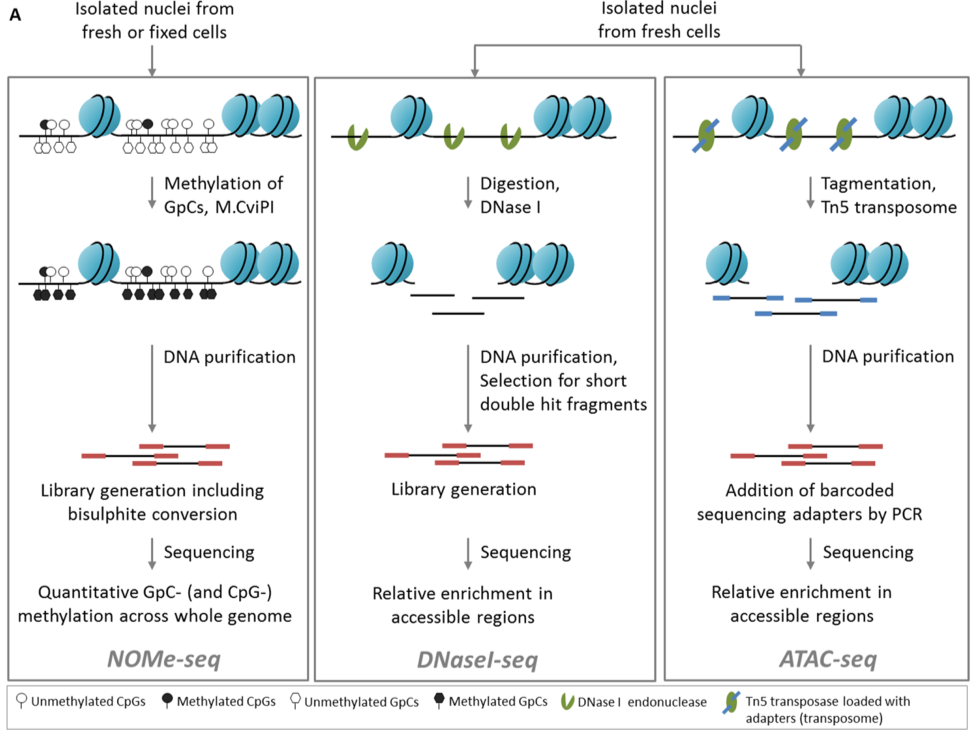
\includegraphics[width=0.75\linewidth]{ChromatinAcc_protocols}
	\caption[]{High-level overview of the workflows for the three main chromatin accessibility assays: NOMe-seq, DNase-seq and ATAC-seq. Reprinted from \cite{Nordstrom2019} with minor modifications.}
	\label{fig:ChromatinAcc_protocols}
\end{figure}

As with DNA methylation, single-cell profiling methods for chromatin accessibility also emerged from its bulk counterparts, including ATAC-seq \cite{Buenrostro2015a}, NOMe-seq \cite{Pott2016} and DNase-seq \cite{Jin2015}. Due to its cost-effective strategy, single-cell ATAC-seq (scATAC-seq) has become the most popular technique to map open chromatin \cite{Cusanovich2015,Cao2018,Chen2018}. Compared to bulk ATAC-seq, scATAC-seq libraries are notably sparse. In a saturated library, \cite{Cusanovich2015} reported a range of $\approx$ 500 to $\approx$ 70,000 mapped reads per cell, with a median of $\approx$ 2500. As the authors report, this represents less than 25\% of the molecular complexity expected from 500-cell bulk experiments. Yet, despite the low coverage, the authors showed that cell-type mixtures can be confidently deconvoluted. Later, in a pioneer effort, \cite{Cusanovich2018b} generated an atlas of chromatin accessibility for different mouse tissues, defining the first \textit{in vivo} landscape of the regulatory genome single-cell resolution.

%- DISCUSS SCALABILITY OF ATAC-SEQ VS NOME-SEQ
% However, the sparse nature of scATAC-seq makes it impractical for the study of heterogeneity in individual regulatory elements. This is addressed mostly by NOMe-seq, which at the expensive of more expensive sequencing and limited scalability, it provides base-pair resolution readouts, even at the single cell resolution \cite{Pott2016}.


\subsection{Multi-modal single-cell sequencing} \label{section:single_cell_multi_modal}

Cellular phenotypes result from the combination of multiple sources of biological information. Undoubtedly, no single "-omics" technology can capture the intricacy of complex molecular mechanisms, but the collective information has the potential to draw a more comprehensive picture of biological processes \cite{Hasin2017,Ritchie2015}.

The profiling of multi-omic readouts at the bulk level is relatively simple, as the same tissue can be dissociated into different aliquots, where each assay can be performed independently \cite{Ritchie2015}. This strategy is also used with single-cell assays, but it has the important downside that the different molecular layers cannot be unambiguously matched, hence limiting the insights that can be inferred from the data. The ultimate goal in single-cell sequencing is to obtain multiple molecular readouts from the same cell, what is called single-cell multi-omics. The development of these technologies will help us understand the fundamental regulatory principles that connect the different molecular layers. In addition, integrative analyses that simultaneously pool information across multiple data modalities (-omics) and across multiple studies promise to deliver a more comprehensive insights into the complex variation that underlies cellular populations .

Notably, the early success and rapid development of single-cell multi-modal methods has led to their recognition as Method of the year in 2019 by the journal \textit{Nature Methods} \cite{NatMethods2020}. However, their development is still in pilot stages and there is no commercial platform available, limiting its widespread use by the community. As reviewed in \cite{Stuart2019,Chappell2018}, multi-modal measurements can be obtained using three broad strategies:
\begin{itemize}
	
	\item \textbf{Application of a non-destructive assay before a destructive assay}: a prominent example is the sorting of cells based on protein surface markers using (multiparameter) fluorescence-activated cell sorting (FACS) followed by high-throughput sequencing \cite{Paul2015}. Although simple and efficient, this approach requires prior knowledge of protein surface markers, and is limited by the spectral overlap of fluorescence reporters.

	\item \textbf{Physical isolation of different cellular fractions followed by high-throughput sequencing}: this technique was pioneered with the introduction of genome and transcriptome sequencing (G\&T-seq) \cite{Macaulay2015}. After cell lysis, the mRNA fraction is separated from the genomic DNA fraction using biotinylated or paramagnetic oligo(dT) beads, followed by the independent sequencing of the mRNA and the DNA. This strategy allows the simultaneous profiling of transcriptomic measurements with (epi)-genomic measurements, including DNA sequence, copy number variation, DNA methylation or chromatin accessibility \cite{Macaulay2015,Hou2016,Angermueller2016,Hu2016}.

	\item \textbf{Conversion of different molecular layers to a common format that can be measured using the same readout}: prominent examples are the simultaneous measure of surface proteins and mRNA expression as in Cellular indexing of transcriptomes and epitopes by sequencing (CITE-seq \cite{Stoeckius2017}) and RNA expression and protein sequencing assay (REAP-seq \cite{Peterson2017}). The idea is to incubate cells with antibodies tagged with oligonucleotides that target specific protein surface proteins. This allows both protein surface markers and mRNA levels to be simultaneously measured using a single sequencing round. Notably, this strategy is significantly more powerful than FACS, as the DNA barcodes can be resolved at the sequence level with much higher sensitivity. A second prominent example is NOMe-seq, described in \Cref{section:chromatin_accessibility}. By labelling accessibile GpC sites with DNA methylation marks, one can simultaneously measure endogenous DNA methylation and chromatin accessibility using a single bisulfite sequencing assay.
\end{itemize}

Although single-cell multi-modal have proven successful, they still face numerous difficulties, both from the experimental and the computational front, including limited scalability, low coverage and high levels of technical noise. These difficulties, also inherent to single-cell uni-modal techniques, generally get exacerbated when doing multi-modal profiling. Quoting Cole Trapnell, one of the pioneers of single-cell data analysis: \textit{When you do a multi-omic assay, you're combining all the bad things from multiple protocols} \cite{Eisenstein2020}. One of the biggest challenge in integrative multi-modal analysis is to develop statistical frameworks that are capable of uncovering biological signal across multiple data modalities while overcoming the technical biases and missing information that are inherent to single-cell experiments. 

A clear example of these challenges is sci-CAR \cite{Cao2018a}, a combinatorial indexing strategy that combines scRNA-seq and scATAC-seq to profile gene expression and chromatin accessibility in the same cell. This is a promising approaches that reported, for the first time, the profiling of both modalities in thousands of cells. However, the  chromatin accessibility modality yielded $\approx$ 10-fold less complexity than (already sparse) scATAC-seq experiments.

I envision that a significant effort will be placed in the next few years to obtain more scalable and cheaper multi-modal measurements from single cells. However, as cost and scalability remain a barrier for high-resolution multi-modal technologies, the use of computational methods that integrate multi-modal measurements from different sets of cells will likely remain a cornerstone of data analysis.


\section{Single-cell data analysis}

From the computational perspective, the rapid development of single-cell technologies has introduced unprecedented challenges for the statistical community, and novel computational methods need to be developed (or adapted) for interrogating the data generated \cite{Stegle2015}. The vast majority of methods are focused on RNA expression, spanning multiple tasks that include normalisation \cite{Lun2016a}, feature selection \cite{Townes2019}, differential expression \cite{Kharchenko2014}, clustering \cite{Kiselev2017}, cell type recognition \cite{Abdelaal2019}, pseudotime inference \cite{Haghverdi2016}, detection of gene regulatory networks \cite{Aibar2017} and batch correction \cite{Haghverdi2018}, among others. Analysis tools have been wrapped into popular platforms such as \textit{Seurat} \cite{Butler2018}, the \textit{Bioconductor class} \textit{SingleCellExperiment} \cite{Amezquita2020} and \textit{Scanpy} \cite{Wolf2018}.

In this section I will provide a brief overview of a typical scRNA-seq analysis pipeline, paying particular attention to the methods that I have used throughout this thesis.

\subsection{Read alignment and gene expression quantification}

The first step in the computational pipeline is to demultiplex the DNA barcodes in order to identify reads that originate from the same cell. This is particularly important when multiple experiments are pooled into a common sequencing library. This task is significantly more complex than in bulk data, owing to the large number of cells and the high rates of errors that can introduce nucleotide missmatches \cite{Tambe2019}.

Subsequently, trimmed reads are aligned to the appropriate reference transcriptome. Gene expression is represented as an integer matrix of counts, with rows representing genomic features (typically genes) and the columns representing individual cells. 

\subsection{Quality control}

Incomplete cell lysis or failures during library preparation may result in poor quality cells that need to be removed for a successful downstream analysis. Typical quality control metrics are the total number of reads detected per cell, the number of genes expressed and the fraction of mitochondrial genes. Cells that are outliers for some of these metrics are filtered out. Importantly, even though there is a generic strategy to assess the quality control for scRNA-seq samples, the specific thresholds vary between data sets and technologies, and care must be taken to always visualise the quality control metrics \cite{Luecken2019}.

A common source of technical variability in single-cell experiments is the existence of doublets, which occurs when more than one cell colocate in the same well or in the same droplet and are thus assigned the same cell barcode. This results in cells that appear as mixtures of different cellular populations and can be mistaken for non-existing intermediate populations or transitory states.  Thus, it is important to remove doublets so that they do not compromise the downstream analysis. In small-scale plate-based technologies, most doublets can be excluded simply by microscope inspection, but in large-scale droplet-based technologies one needs to adopt data-driven heuristics to exclude multiplet libraries \cite{McGinnis2019}. 


\subsection{Normalisation}

The first step of quality control is essential to remove poor quality cells, but the quality control metrics can vary widely even between cells that pass the filtering criteria. These sources of technical variation arise from any of the library preparation steps, and includes PCR amplification biases, differences in RNA capture and reverse transcription efficiency, among others. In addition, the stochasticity of the amplification process produces dropout events, in which no read counts are observed for genes that are expressed \cite{VandenBerge2018}. This does not tend to be a problem for highly-expressed genes, but it poses a major challenge for lowly expressed genes.

Data normalisation steps are mandatory to eliminate (or at least reduce) the technical variation. Methods that were developed for bulk RNA-seq, including \textit{TMM} \cite{Robinson2010} and \textit{DEseq2} \cite{Love2014} are not successful for scRNA-seq owing to large number of zeros that dominate the gene expression matrix.

In this thesis I adopted the methodology implemented in the \textit{scran} package \cite{Lun2016a}. Briefly, this normalisation procedure divides the gene counts by a size factor per cell and subsequently applies a log transformation with pseudocount on each observation. The essential innovation for single-cell data is to pool expression values from multiple cells (resulting in less zeros) and subsequently deconvolves the cell-specific size factors using a linear system of equations.

Recent works have suggested that global size factors do not effectively normalise all genes at the same time, and different groups of genes require specific size factors in order to remove technical biases \cite{Hafemeister2019}. In this thesis I have not explored this approach, but it showcases how data normalisation is still an open and debated topic in scRNA-seq.

\subsection{Dimensionality reduction}

A key principle of biological data sets is that covariation patterns between the features (i.e. genes) results from differences in underlying processes that can be inferred and interpreted. This key assumption sets off an entire statistical framework of exploiting the redundancy encoded in the data set to reduce the dimensionality of the data in an unsupervised fashion.

Principal Component Analysis (PCA) is the most popular technique for dimensionality reduction of scRNA-seq data \cite{Luecken2019}. A typical analysis pipeline performs clustering, graph inference and other downstream analyses on the (denoised) latent PCA space defined by the top N principal components (where components are ranked by variance explained). Importantly, by maximising the variance explained, PCA implicitly assumes a normal distribution for each feature, and it therefore requires the log transformation above to turn integer counts into continuous measurements. In addition, the log transformation prevents signal being driven by a small number of extremely highly-expressed genes (because in the raw counts the variance of each gene is proportional to its mean expression). 

PCA defines a linear transformation from the high-dimensional space to the low-dimensional space where each component captures an orthogonal source of variation. Capturing the biological signal in most single-cell data sets require a relatively high number of components. Unfortunately, humans do not have the ability to make visual representations of more than three dimensions at the same time, so further dimensionality reduction is typically applied using non-linear techniques, including t-Distributed Stochastic Neighbor Embedding (t-SNE) \cite{vanDerMaaten2008} and Uniform Manifold Approximation and Projection (UMAP) \cite{McInnes2018}. Both methods have been extensively applied, although UMAP is gaining popularity for larger data sets because it preserves better the global structure, whereas t-SNE is largely aimed at preserving local structure. 

\subsection{Clustering}

Unsupervised clustering is arguably one of the most powerful application of single-cell genomics, as it underpins the ability to define cell types in a coherent, systematic and unbiased manner. Although clustering is still largely empirical and no strong consensus exists on the methodology and the parameters, it is applied in virtually any single-cell data set in one form or another \cite{Kiselev2019}. The most popular clustering algorithm has traditionally been k-means, which iteratively identifies $k$ cluster centroids, and assigns each cell to the nearest centroid. This method is simple, fast and efficient for medium-sized data sets. For large-scale data sets, however, the use of community-detection algorithms on coarse-grained graphs has become more popular. Briefly, the first step of commnity-detection methods is to build a k-nearest-neigbourhood graph using a cell-to-cell similarity metric, where each node corresponds to one cell. Then, tighly connected communities are detected by maximising a modularity score, where the modularity quantifies the assignment of nodes to communities when contrasted to a random network.

\subsection{Inference of developmental trajectories}

In many biological systems, and particularly during embryonic development, cells display a continuous spectrum of states where discretisation by clustering may be inappropriate. Due to the destructive nature of single-cell assays, experiments are limited to snapshots and thus are not capable of measuring continuous time. However, differentiating cells are typically asynchronised and display a continuous spectrum of molecular states that reflect the underlying trajectory. Computational methods have been developed to reconstruct this continuity using latent mathematical representations, and are often called pseudotime methods \cite{Saelens2019}. The aim of pseudotime methods is to generate an ordination of cells according to some metric, which is usually (but not necessarily) some approximation of real time that is inferred from the data. A myriad of pseudotime methods have been developed, with tailored assumptions depending on the nature of the input data and the expected topology of the trajectory (linear, bifurcating, etc.), among other variables \cite{Saelens2019}. 

\section{Integrative analysis of single-cell omics}

Despite the explosion of statistical methods for scRNA-seq data analysis, to date only a few methods have been published with the aim of performing data integration across experiments and data modalities. This is currently defined as one of the grand challenges in single-cell data science \cite{Lahnemann2020}.

\subsection{Defining the common coordinate framework}

The first step when performing data integration is to consider a common coordinate framework to anchor the different data modalities. This defines three broad types of strategies for data integration (\Cref{fig:overview_data_integration}): 

\begin{itemize}

	\item Cells as the common coordinate (vertical integration): when the different data modalities are derived from the same cell in \textit{matched} multi-omic assays. This is exemplified by assays such as single-cell Methylome \& Transcriptome (scM\&T-seq) \cite{Angermueller2016}, Cellular Indexing of Transcriptomes and Epitopes by sequencing (CITE-seq) \cite{Stoeckius2017} or Single-nucleus chromatin accessibility and RNA expression sequencing (SHARE-seq) \cite{Ma2020}.

	\item Genomic features as the common coordinate framework (horizontal integration): when multiple data modalities of the same type are derived from different subsets of cells. We call this \textit{non-matched} multi-omics and the main advantage is that it is significantly easier and cheaper to obtain than \textit{matched} multi-omics, and as a result most of the current data sets to date belong to this category. An example could be the profiling of scRNA-seq experiments from cells from the same tissue across different groups of donors, where the set of genes represents the anchors.

	\item No common coordinate framework in the high-dimensional space (diagonal integration): when both cells and genomic features are different between experiments. This is exemplified by profiling RNA expression and chromatin accessibility from independent sets of cells.

\end{itemize}

\begin{figure}[H]
	\centering
	\includegraphics[width=0.75\linewidth]{overview_data_integration}
	\caption{\textbf{Defining the data integration strategy: choosing the common coordinate framework}.\\Schematic representation of (a) Horizontal integration, when features act as anchors (b) Vertical integration, when cells act as anchors (c) Diagonal integration, when no anchors exist. }
	\label{fig:overview_data_integration}
\end{figure}

\subsection{Challenges of data integration}

The joint analysis of multiple data sources must tackle numerous challenges, some of which are:

\begin{itemize}
	\item \textbf{Heterogeneous data modalities}: measurements collected using different techniques generally exhibit heterogeneous statistical properties and have to be modelled under different statistical assumptions. For example, combining count (i.e. gene expression) and binary traits (i.e.somatic mutations) under the same statistical framework is not a trivial task. In the statistics community, this is commonly refered to as the multi-view learning problem \cite{Xu2013,Li2016}.

	\item \textbf{Overfitting}: as the number of molecular layers increase but the number of samples remain limited, modelling strategies need to account for the risk of overfitting, which can lead to poor generalisation performance. For example, scM\&T-seq captures the methylation status for potentially millions of CpG sites, but the experimental designs are typically restricted to only a few hundred cells. This is a classic case of a large p and small n problem in high-dimensional statistics, which poses important challenges for most statistical inference procedures.

	\item \textbf{Undesired sources of heterogeneity}: multi-omics data sets typically contain undesired sources of heterogeneity, both technical and biological \cite{Ritchie2015}. Prominent examples are batch effects or cell cycle variation, respectively. If not accounted for, such strong sources of variability can hidden the signal of interest \cite{Buettner2015}. Therefore, understanding and correcting for the underlying principal components of the data represent a critical step before other computational pipelines are applied \cite{Meng2016}.

	\item \textbf{Missing data}: a major problem in some single-cell methodologies is the large amounts of missing information. For example, in a typical single-cell bisulfite experiment less than 10\% of all CpG sites in the genome are measured \cite{Smallwood2014}. This imposes important challenges to some of the conventional statistical methods that do not handle missing information. Furthermore, different assays differ on how missing data is defined. For bisulfite sequencing methods, the missing values are clearly distinguishable from the observed values. However, for other methods such as scRNA-seq or scATAC-seq, the absence of sequence reads do not distinguish between the event that the genomic feature was not measured from that the readout was indeed zero \cite{Clark2018}. Handling of missing information is an important aspect of multi-omics data integration, as some of the conventional statistical methods that do not handle missing information, including linear regression or principal component analysis.

	\item \textbf{Delineating biological vs technical noise}: multi-omics datasets from relatively complex experimental designs typically contain multiple sources of heterogeneity, both technical and biological. If not accounted for, technical variability can mask biological signal of interest \cite{Buettner2015}. Understanding and correcting technical variation is a critical step to ensure a successful computational analysis.

	\item \textbf{Scalability}: as sequencing costs decrease and technologies improve, we anticipate that multi-modal data sets will follow a similar trend as scRNA-seq, where in the span of less than ten years the size of the experiments ranged from the order of tens to milions of cells \cite{Svensson2018}. The interrogation of exceptionally large data sets requires computational methods to scale accordingly.

	\item \textbf{Noise}: because of the small amounts of starting material, single-cell technologies are inherently noisy and result in large amounts of technical noise \cite{Stegle2015}. Hence, in most cases, inspection of individual genes or cells tends to be unreliable. To overcome this challenge, computational frameworks are required to leverage information on the similarities between cells and/or genes to delinate the signal from noise in order to obtain reliable estimates \cite{Vallejos2015}. Prominent examples are (empirical) Bayesian approaches that are able to borrow information across cells and/or genes and propagate uncertainity when doing inference and predictions \cite{Kharchenko2014}.

	% \item \textbf{Data-driven hypothesis}: the exponential accumulation of biological data is empowering a new type of scientific method where the sheer data itself guides the researcher to formulate specific hypothesis. Importantly, rather than inverting the direction of the scientific method from data to hypothesis, the exploitation of the information hidden in big data sets has the potential to make this relationship bidirectional. Consequently, there is a growing interest in the use of unsupervised methods that, under some specific (hypothesis-driven) assumptions, are able to extract biological insights from the data.

	\item \textbf{Principled validation of the model outputs}: The assessment of data integration outputs is one of the most challenging steps. For most cases, no ground truth is available and one has to assess the model fit by relying on quality control statistics and/or assessing the impact of the integration on downstream analysis tasks (i.e. differential expression, dimensionality reduction, clustering, etc.). The evaluation of the model fit is particularly hard for non-linear methods that can be prone to overfit. 

\end{itemize}

\subsection{Defining the methodology}

Once the common coordinate framework is defined, one needs to choose the data integration strategy. These can fall into two classes: \textit{local} and \textit{global}, a notation inspired from integrative approaches that have been pursued at the bulk level \cite{Ritchie2015}. 

\textit{Local} analyses refer to associations between specific features across different molecular layers, with the aim of detecting putative interactions between them. Prominent examples are associations between genetic variants and gene expression (expression quantitative trait loci, eQTL) or correlations between the epigenetic status of putative regulatory elements and gene expression of nearby genes. The restriction to a local search space is often necessary, to maintain the problem tractable. For example, cis eQTL mapping is most prevalent because by testing only proximal genetic variants for each gene, the effects of the multiple testing burden is reduced \cite{Nica2013}. Since such association analyses are typically performed per feature (across cells), \textit{local} analyses generally requires unambiguous matching between the modalities, as given only by \textit{matched} multi-modal assays, and thus belongs to the category of vertical analysis. As for methods, most \textit{local} analyses rely on different flavours of linear regression models, with different modelling assumptions depending on the nature of the molecular readouts. This can include non-gaussian likelihoods, sparsity assumptions to prevent overfitting or probabilistic terms to account for random effects. For example, linear mixed models (LMMs) are a popular framework for performing genetic analyses \cite{Moore2019}. In a LMM, a random effect term is added to account for the population structure and relatedness between individuals, which may affect both the phenotype and the genotype, thus leading to spurious associations if not accounted for.

While useful for characterising genetic variants or identifying putative regulatory elements, \textit{local} analyses have limited capacity to discover complex maps of molecular heterogeneity that result from interactions between genomic features. An alternative strategy for data integration is to exploit the full spectrum of measurements to identify cellular states defined by the coordinated action of multiple genomic elements. For example, cell cycle phase or pluripotency potential are cellular properties that are determined by gene regulatory networks and thus cannot be studied with \textit{local} analyses. \textit{Global} integration is typically (but not always) performed using unsupervised dimensionality reduction approaches that find common modes of variation between molecular layers. Alternatives have been proposed that perform transformations on each data type before merging them into a common similarity network, e.g. using kernel or graph-based approaches \cite{Lanckriet2004, Wang2014}. Nonetheless, both of these approaches have important limitations that will be discussed in this thesis.

Popular examples of global integration methods that have been adapted from the statistical literature are derived as different flavours of matrix factorisation: PCA, Canonical Correlation Analysis (CCA, implemented in Seurat \cite{Butler2018}), Group Factor Analysis (MOFA \cite{Argelaguet2018,Argelaguet2019}, which is introduced in this thesis), Projected Least Squares (PLS, implemented in DIABLO \cite{Singh2018}) and Non-negative Matrix factorisation (NMF, implemented in LIGER \cite{Welch2019}), among others. Although all of these methods share important similarities, the statistical assumptions underlying each model are heavily dependent on the common coordinate framework adopted. As such, the output of each data integration model has specific assumptions, challenges and diagnostics that must be adopted accordingly.

\subsubsection{Horizontal integration}

Horizontal integration strategies define features as the common anchors in \textit{unmatched} experiments of the same type. This task is faced in most large-scale scRNA projects where data is generated across multiple batches, as uncontrollable differences in the experimental procedure result in systematic deviations in the observed RNA expression (or even cell type composition) across the different batches. If left unaccounted for, these sources of technical variation can mask relevant biological variability and thus complicate the interpretation of the downstream analysis. Horizontal integration is currently the most common integrative task, and it is typically regarded as a batch correction problem, where the aim is to remove undesired technical variation across batches while preserving the biological variation contained within each batch \cite{Tran2020}. With the growing availability of reference atlases, epitomised by the Human Cell Atlas project \cite{Aviv2017}, this is arguably one of the most important steps in a single-cell analysis pipeline. 

Linear batch correction methods that were originally developed for bulk datasets such as \textit{limma} \cite{Ritchie2015b} and \textit{ComBat} \cite{Johnson2006}) are not successful for single-cell experiments, mainly because they assume identical (or at least, known) cell type composition across batches. In practice, however, the abundance of cellular subpopulations can vary even between biological replicates due to subtle differences in the library preparation. As a consequence, the majority of horizontal integration methods developed for single-cell data rely on non-linear (or locally linear) strategies that account for differences in cell type compositions.

Several integrative methods have been developed and benchmarked. This includes MNN \cite{Haghverdi2018}, Seurat \cite{Butler2018}, LIGER \cite{Welch2019}, Harmony \cite{Korsunsky2019}, BBKNN \cite{Polanski2019}, scVI \cite{Lopez2018}, Conos \cite{Barkas2019}, among others, which have been benchmarked in an independent study \cite{Luecken2020}. Despite sharing similar principles, these each employ different methodologies. In particular, MNN and Seurat v3 detect mutual nearest neighbors in a joint low-dimensional space, defined by either principal components (MNN) or canonical covariates (Seurat v3). Instead, LIGER performs integrative NMF and disentangles dataset-specific factors versus shared factors, followed by the construction of a neighborhood graph using the shared factors. Harmony learns a cell-specific linear correction function by successive rounds of k-means clustering on a principal component space. BBKNN performs correction on a neighbourhood graph, which results in much faster computations at the expense of losing single-cell resolution. Finally, scVI is a Bayesian variational autoencoder with a probabilistic formulation which includes random variables that account for batch-specific variation.

Most of these methods also share a common set of challenges. First, a classical problem of non-linear integration methods is over-correction, which occurs when the batch correction vector is wrongly estimated and the algorithm forcibly merges non-matching subpopulations of cells \cite{Luecken2020}. This can occur for example when no shared axes of biological variation are preserved between the datasets. An optimal method should be able to detect this and prevent a merging of datasets when no biological variation exists. Second, most methods perform data integration in a denoised latent space, typically using principal components or canonical covariates. This step undoubtedly improves most batch correction algorithms, and is extremely useful for some downstream analysis tasks such as manifold embedding (t-SNE or UMAP plots), graph inference and clustering. However, the high-dimensional observations (i.e. the gene expression counts) can be severely distorted as a result of the batch alignment, and other downstream gene-based analyses such as gene marker detection or differential expression analysis can be problematic \cite{Haghverdi2018}.

\subsubsection{Vertical integration}

Vertical integration strategies take advantage of the unambiguous assignment between the molecular profiles in \textit{matched} multi-modal experiments and thus define cells as anchors between data modalities. This facilitates the detection of co-variation patterns across features and permits two data integration strategies: gene-based \textit{local} analysis and a cell-based \textit{global} analysis.

\textbf{Local analysis}

In \textit{local} analyses, the challenge is to distinguish true interactions between features from spurious associations that can result from global confounding effects. To correct for global confounding effects (both technical and biological) affecting the expression phenotype in eQTL mapping, methods such as Principal Component Analysis and PEER \cite{Stegle2010} are often used to identify factors that capture global expression trends, which can be added as covariates in the linear (mixed) model framework. Similarly, the use of a kinship matrix is used to account for global genotype effects that result from population substructure and individual relatedness. Mapping eQTLs using single-cell genomics has led to the identification of cell type-specific eQTL in rare cell populations, which would have been masked using bulk assays \cite{VanDerWijst2018}. Additionally, \cite{Cuomo2020} combined differentiations of iPSCs across multiple donors and single cell expression profiles to show how eQTL influence expression dynamically along a differentiation trajectory. Single cell eQTL mapping is growing as a field, and it promises to provide an extra layer to our understanding of genetic regulation at the molecular level. As methods to assay various molecular traits at single cell resolution become more established, non-expression single cell QTL mapping, where genomic variants are associated with changes in DNA methylation (mQTL), histone modifications (hQTL) or protein (pQTL) level at single cell resolution may also become routine.

\textbf{Global analysis}

% A key principle of biological data is that at least some of the variation observed in the molecular measurements results from differences in underlying, often unobserved, processes. Such processes, whether driven by biological or technical effects, are manifested by coordinated changes in multiple features and thus could be retrieved by learning useful mathematical representations that can be linked to the latent biological processes.

When having a single data modality, PCA is the paradigmatic method for global analysis, and will be discussed in more detail in Chapter 3. Briefly, PCA infers an orthogonal projection of the data onto a low-dimensional space such that the variance explained by the projected data is maximised. The key for the popularity of PCA is its linearity assumption, which ensures that the resulting principal components are simple and interpretable. PCA has also been applied as an integrative method for multi-modal data by extracting principal components from each modality and subsequently comparing them. This approach was attempted in one of the first multi-modal datasets, where scM\&T-seq was used to simultaneously profile RNA expression and DNA methylation on 61 embryonic stem cells \cite{Angermueller2016}. The authors found that a small number of PCs derived from mRNA expression displayed significant correlations with PCs derived from DNA methylation, which suggests that some global sources of variation are preserved across data modalities, but a large fraction of the variation is uncorrelated. This simple analysis provides the intuition for some of the more advanced multi-omic integration methods aimed at performing variance decomposition across data modalities.

An alternative strategy has been to apply PCA after concatenation of the datasets, but this has important limitations when applied to datasets where the features are structured into non-overlapping views (referred to as multi-view data in the machine learning literature). First, PCA extracts components that maximise the variance explained, but it is difficult to quantify the contribution that each component has from each data modality. Second, in its vanilla implementation, PCA does not handle missing values and hence imputation is required when cells do not have measurements available in all data modalities. This is a frequent problem in \textit{matched assays}, as cells might pass quality control for one data modality but not the other. Third, by maximising the variance explained, PCA implicitly assumes a normal distribution for each feature, and is not well suited for the integration of binary and count-based readouts. 

Generalisations of PCA for the integration of multi-omics data have been devised by adapting multi-view learning methods from the statistics literature. Although most of these methods were originally devised for bulk data, the majority of them remain applicable to single-cell multi-modal data. This includes MOFA \cite{Argelaguet2018}, JIVE \cite{Lock2013}, PLS \cite{Singh2018}, MCIA \cite{Meng2014} and iNMF \cite{Welch2019}, all being unsupervised dimensionality reduction methods derived as different flavours of matrix factorisation. As I will discuss in this thesis, the matrix factorisation framework is very appealing due to its simplicity, interpretability, scalability and limited overfitting. Also, it has shown to be an excellent choice for extracting interpretable signatures from sparse and noisy observations such as single-cell measurements.


\subsubsection{Diagonal integration}

The third type of data integration problem is faced when no common coordinate framework exists in the high-dimensional space. This task is faced in \textit{unmatched} experiments when different molecular layers are profiled in different subsets of cells, and is arguably the hardest type of integration. Diagonal integration methods are generally aimed at reconstructing a low-dimensional manifold that captures co-variation across data modalities. Thus, a critical assumption of this integrative strategy is the existence of a latent manifold that is shared between the data modalities. For example, this could represent cells sampled from a common differentiation trajectory or cells sampled from a common set of discrete subpopulations.

The simplest strategy that has been employed to solve a diagonal integration task is to transform it into a simpler horizontal integration task. This can be achieved by summarising molecular measurements over genomic elements that can be unambiguously linked (i.e. RNA expression and promoters methylation). Using this strategy, horizontal methods such as LIGER \cite{Welch2019} and Seurat \cite{Stuart2019b} have been successful at integrating unmatched epigenetic and transcriptomic experiments from the same tissue, and even across different species. However, this strategy relies on fragile biological assumptions and is prone to fail in scenarios where molecular layers are not strongly correlated. A good example is early embryonic development where promoter DNA methylation and/or chromatin accessibility are not as predictive of RNA expression \cite{Argelaguet2019} as in terminally differentiated cell types. 

Alternatively, a few methods have attempted to solve this problem by reconstructing technology-invariant integrated latent spaces. The first method to be developed was MATCHER \cite{Welch2017}, a gaussian process latent variable model. However, this method relies upon the strong assumption that biological variation is defined by a unidimensional axis of variation. Some recent methods, including MMD-MA \cite{Liu2019a}, SCIM \cite{Stark2020} and UnionCom \cite{Cao2020} have generalised MATCHER to account for complex multivariate trajectories. However, no independent benchmarking has yet been performed, and the biological insights extracted from these methods have been relatively limited. 


\section{Thesis overview}

In this PhD thesis I sought to develop computational strategies for data integration in the context of single-cell multi-omics. In particular my research focused on the vertical integration task, where cells are the common coordinate framework in \textit{matched} assays.

In Chapter 2 I introduce single-cell nucleosome, methylation and transcription sequencing (scNMT-seq), an experimental protocol for the genome-wide profiling of RNA expression, DNA methylation and chromatin accessibility in single cells. While some approaches have reported unbiased genome-wide measurements of up to two molecular layers, scNMT-seq allows, for the first time, the simultaneous profiling of three molecular layers at single cell resolution. We validate the readouts using a simple prototype experiment, and we show how scNMT-seq can be used to study coordinated epigenetic and transcriptomic heterogeneity along a simple differentiation process.

In Chapter 3 I present Multi-Omics Factor Analysis (MOFA), a statistical framework for the integration of multi-omics data sets. MOFA is a latent variable model that offers a principled approach to explore, in a completely unsupervised manner, the underlying sources of sample heterogeneity in a multi-omics data set. Once the model is trained, the inferred low-dimensional space can be interpreted using a tool-kit of downstream analysis procedures that include visualisations, clustering, imputation or prediction of clinical outcomes. First, we validate the different model features using simulated data. Second, we apply MOFA to a multi-omics study of 200 chronic lymphocytic leukaemia patients. In a quick unsupervised analysis, MOFA revealed the most important dimensions of disease heterogeneity, connected to clinical markers that are commonly used in practice. In a second application we show how MOFA can cope with noisy single-cell multi-modal data, identifying coordinated transcriptional and epigenetic changes along a differentiation process.

In Chapter 4 I discuss how we combined scNMT-seq and MOFA to study the role of epigenetic layers during mouse gastrulation, a critical embryonic stage that spans exit from pluripotency to primary germ layer specification. In this study we built the first triple-omics roadmap of mouse gastrulation, which enabled us to perform an integrative study that revealed novel insights on the dynamics of the epigenome. Notably, we show that cells committed to mesoderm and endoderm undergo widespread epigenetic rearrangements, driven by demethylation in enhancer marks and by concerted changes in chromatin accessibility. In contrast, the epigenetic landscape of ectoderm cells remains in a \textit{default} state, resembling earlier stage epiblast cells. This work provides a comprehensive insight into the molecular logic for a hierarchical emergence of the primary germ layers, revealing underlying molecular constituents of the Waddington's landscape.

In Chapter 5 I propose an improved formulation of the MOFA framework aimed at performing integrative analysis of large-scale (single-cell) data sets across multiple studies/conditions as well as data modalities. We introduce key methodological developments, including a fast stochastic variational inference framework and multi-group generalisation in the structure of the prior distributions. All together, this allows MOFA to  disentangle heterogeneity across sample groups (i.e. studies or experimental conditions) and data modalities (i.e. omics) in very large single-cell studies. First, we benchmark the new features of the model using simulated data. Next, we use a single-cell DNA methylation data set of neurons from mouse frontal cortex to demonstrate how from a seemingly unimodal data set, one can investigate hypothesis using a multi-group and multi-view setting. Finally, we apply MOFA to the scNMT-seq data set generated in Chapter 3, revealing underlying sources of molecular variation associated with early cell fate decisions.

Finally, Chapter 6 summarises this thesis and provides an outlook of future research.
